\chapter{Aplicaciones}

En este capítulo usaremos la aplicación descrita en el capítulo anterior en distintos conjuntos de datos.

\section{Cáncer de mama}

En primer lugar, utilizaremos la aplicación con datos el diagnóstico del cáncer de mama. El conjunto de datos ha sido obtenido de~\cite{cancer}. Consta de 699 observaciones y 10 variables (más la variable de clasificación). Éstas son:

\begin{enumerate}
	\item Código de la muestra
	\item Espesor
	\item Uniformidad del tamaño celular
	\item Uniformidad de la forma celular
	\item Adhesión marginal
	\item Tamaño de las células epiteliales
	\item Bare nuclei
	\item Cromatina
	\item Normal Nucleoli
	\item Mitosis
	\item Clase (B = beningno; M = maligno)
\end{enumerate}

Todas las variables toman valores numéricos entre 1 y 10, excepto el número de muestra.\\

Puesto que esta variable no aporta nada, la eliminamos, dejando 10 variables (9 + variable de clasificación).\\

Un subconjunto de los datos se pueden ver en la Figura~\ref{fig:datos_cancer}.

\begin{figure}[tbph!]
\centering
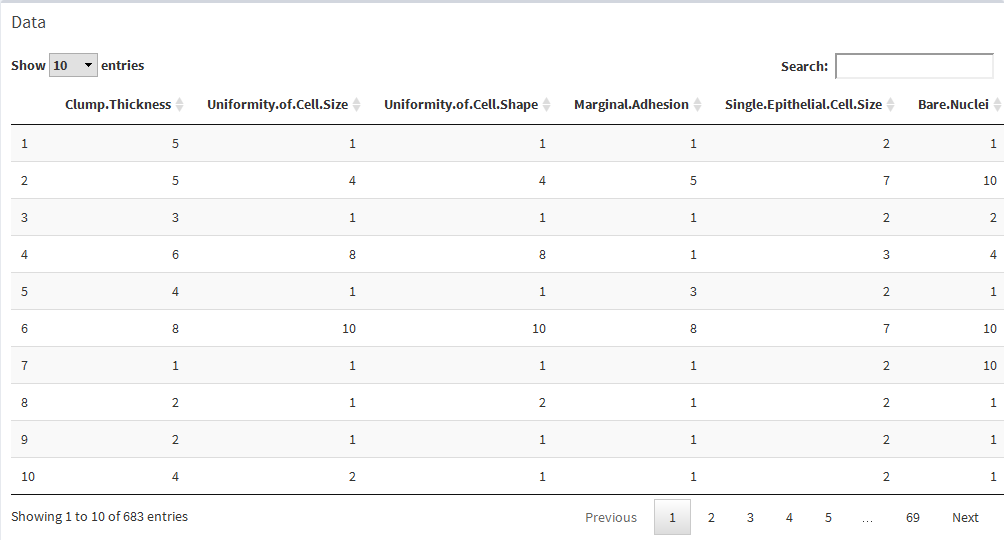
\includegraphics[width=0.5\linewidth]{imagenes/cancer/datos.png}
\caption{Subconjunto de los datos de cáncer de mama}
\label{fig:datos_cancer}
\end{figure}

Con la aplicación podemos ver cuál es la distribución de cada una de las variables. Por ejemplo, en el caso del espesor la distribución por clase de tumor se puede ver en la Figura~\ref{fig:thickness}.\\

\begin{figure}[tbph!]
	\centering
	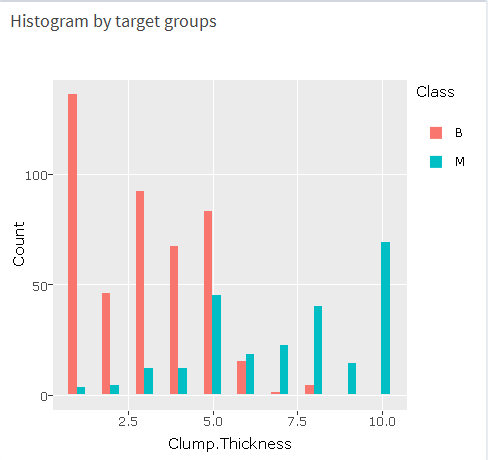
\includegraphics[width=0.5\linewidth]{imagenes/cancer/thickness.png}
	\caption{Distribución del espesor por clase de tumor}
	\label{fig:thickness}
\end{figure}

Se puede observar que la presencia de un espesor menor está presente se da en tumores benignos, y a medida que el espesor es mayor se producen más tumores malignos.\\

\begin{figure}[htbp!]
	\label{fig:cancer_par}
	\begin{center}
		\begin{subfigure}[t]{\textwidth}
			\centering
			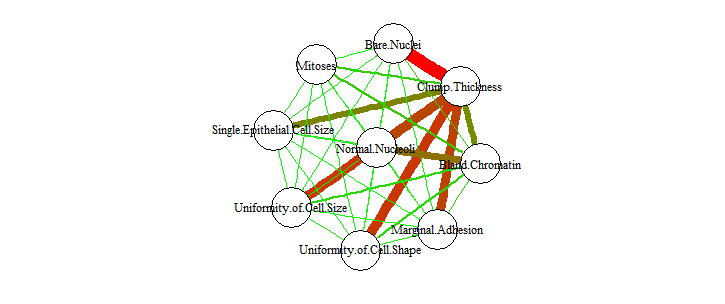
\includegraphics[height=7.5cm]{imagenes/cancer/1.png}
			\caption{Red parenclítica de la observación 1}
		\end{subfigure}
		\begin{subfigure}[t]{\textwidth}
			\centering
			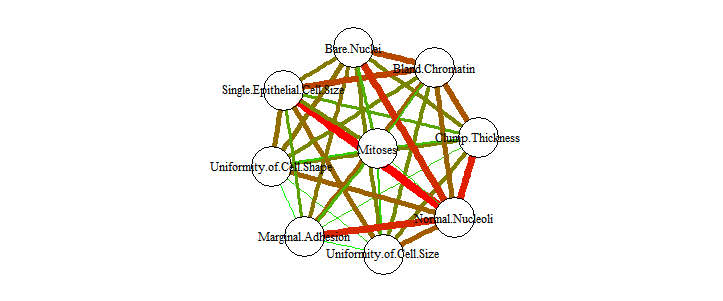
\includegraphics[height=7.5cm]{imagenes/cancer/2.png}
			\caption{Red parenclítica de la observación 2}
		\end{subfigure}
		
	\end{center}
	\caption{Redes parenclíticas con modelo de regresión lineal}
\end{figure}
 
En la Figura~\ref{fig:cancer_par} se pueden observar las redes parenclíticas de las dos primeras observaciones obtenidas con el modelo lineal.\\

Podemos ver si existen diferencias entre las redes parenclíticas de las observaciones con tumores benignos y malignos. La Figura~\ref{fig:cancer_diferencias} muestra cuatro observaciones de cada clase de tumor.\\

\begin{figure}[htbp!]
	\label{fig:cancer_diferencias}
	\begin{center}
		\begin{subfigure}[t]{0.2\textwidth}
			\centering
			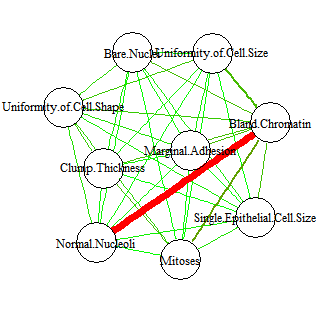
\includegraphics[height=3cm]{imagenes/cancer/b1.png}
			\caption{Obs. 8}
		\end{subfigure}
		\begin{subfigure}[t]{0.2\textwidth}
			\centering
			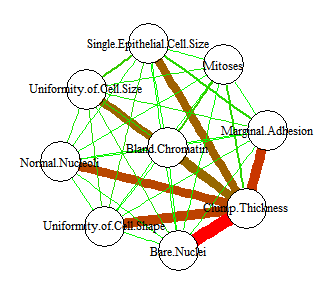
\includegraphics[height=3cm]{imagenes/cancer/b2.png}
			\caption{Obs. 26}
		\end{subfigure}
		\begin{subfigure}[t]{0.2\textwidth}
			\centering
			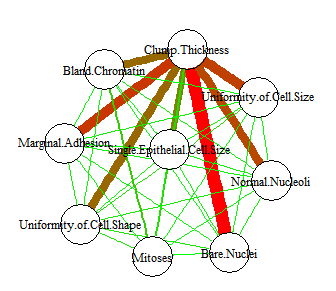
\includegraphics[height=3cm]{imagenes/cancer/b3.png}
			\caption{Obs. 34}
		\end{subfigure}
		\begin{subfigure}[t]{0.2\textwidth}
			\centering
			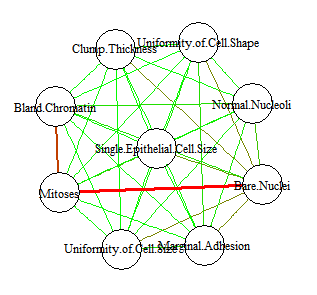
\includegraphics[height=3cm]{imagenes/cancer/b4.png}
			\caption{Obs. 60}
		\end{subfigure}	
		
		\begin{subfigure}[t]{0.2\textwidth}
			\centering
			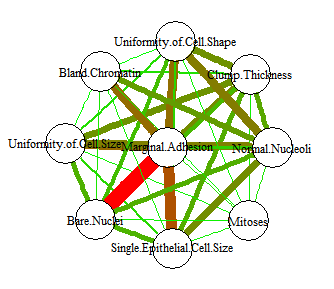
\includegraphics[height=3cm]{imagenes/cancer/m1.png}
			\caption{Obs. 41}
		\end{subfigure}
		\begin{subfigure}[t]{0.2\textwidth}
			\centering
			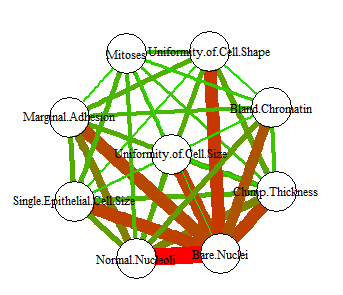
\includegraphics[height=3cm]{imagenes/cancer/m2.png}
			\caption{Obs. 43}
		\end{subfigure}
		\begin{subfigure}[t]{0.2\textwidth}
			\centering
			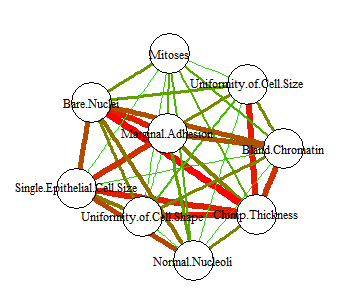
\includegraphics[height=3cm]{imagenes/cancer/m3.png}
			\caption{Obs. 50}
		\end{subfigure}
		\begin{subfigure}[t]{0.2\textwidth}
			\centering
			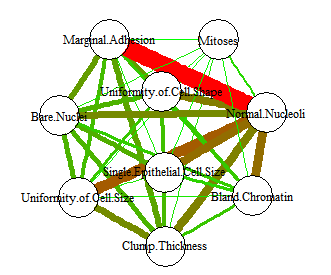
\includegraphics[height=3cm]{imagenes/cancer/m4.png}
			\caption{Obs. 51}
		\end{subfigure}		
	\end{center}
	\caption[Redes parenclíticas por clase de tumor con modelo de regresión lineal]{Redes parenclíticas por clase de tumor con modelo de regresión lineal. En la primera fila se muestran las observaciones con tumor benigno y, en la segunda, con tumor maligno}
\end{figure}

Se puede observar que en el caso de las observaciones con tumor benigno existe un menor peso en las aristas (color verde de las aristas), y en las observaciones con tumor maligno existe un mayor entre las aristas (color rojo de las aristas).\\

Puesto que disponemos de varios modelos de regresión, puede que el modelo lineal no sea el más indicado, por lo que calculamos la regresión para cada uno de los modelos de regresión (lineal, exponencial, cuadrática y recíproca), junto con la de los modelos de machine learning clásicos (árboles de decisión, Support vector Machine y redes neuronales), y calculamos la curva ROC de cada clasificador (Figura~\ref{fig:roc_cancer}).\\

\begin{figure}[tbph!]
	\centering
	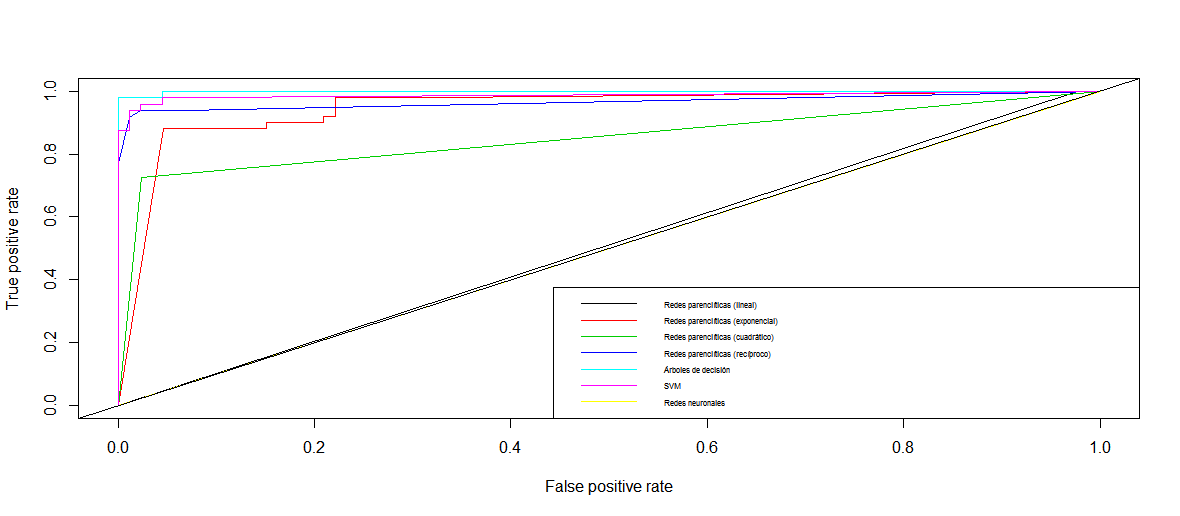
\includegraphics[width=0.9\linewidth]{imagenes/cancer/ROC_cancer.png}
	\caption{Curvas ROC}
	\label{fig:roc_cancer}
\end{figure}

Se puede observar que el mejor clasificador por redes parenclíticas es el obtenido con el modelo de regresión recíproco, seguido del exponencial y el cuadrático. El peor clasificador es el lineal. Respecto a los algoritmos clásicos de machine learning, el mejor clasificador son los árboles de decisión seguido de los Support Vector Machine y de las redes neuronales.\\

Sobre todos los clasificadores, el mejor son los árboles de decisión, seguido de los Support Vector Machine y las redes parenclíticas con modelo recíproco.\\
 
Puesto que el mejor modelo de redes parenclíticas es el modelo recíproco, veamos si existen diferencias entre las redes parenclíticas según la clase de tumor (Figura~\ref{fig:cancer_rec}).\\

\begin{figure}[htbp!]
	\label{fig:cancer_diferencias}
	\begin{center}
		\begin{subfigure}[t]{0.25\textwidth}
			\centering
			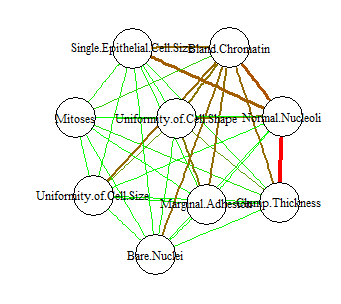
\includegraphics[height=3cm]{imagenes/cancer/b1_reciproco.png}
			\caption{Obs. 8}
		\end{subfigure}
		\begin{subfigure}[t]{0.25\textwidth}
			\centering
			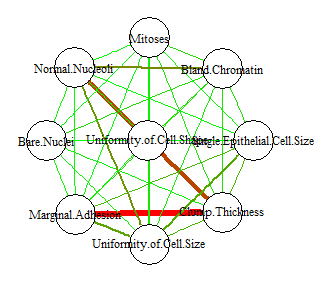
\includegraphics[height=3cm]{imagenes/cancer/b2_reciproco.png}
			\caption{Obs. 26}
		\end{subfigure}
		\begin{subfigure}[t]{0.25\textwidth}
			\centering
			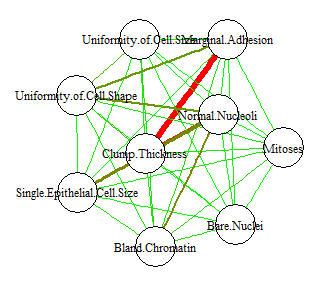
\includegraphics[height=3cm]{imagenes/cancer/b3_reciproco.png}
			\caption{Obs. 34}
		\end{subfigure}
		
		\begin{subfigure}[t]{0.25\textwidth}
			\centering
			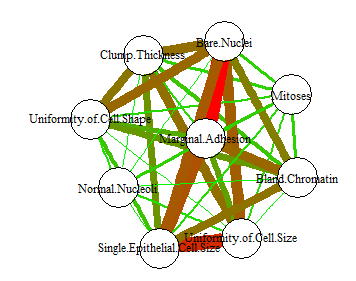
\includegraphics[height=3cm]{imagenes/cancer/m1_reciproco.png}
			\caption{Obs. 41}
		\end{subfigure}
		\begin{subfigure}[t]{0.25\textwidth}
			\centering
			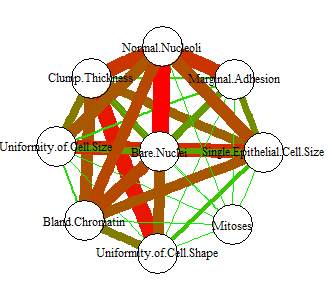
\includegraphics[height=3cm]{imagenes/cancer/m2_reciproco.png}
			\caption{Obs. 43}
		\end{subfigure}
		\begin{subfigure}[t]{0.25\textwidth}
			\centering
			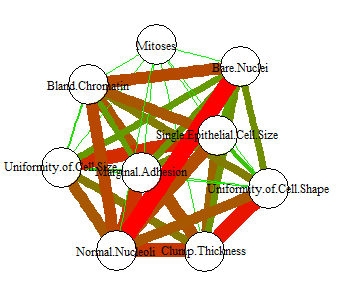
\includegraphics[height=3cm]{imagenes/cancer/m3_reciproco.png}
			\caption{Obs. 50}
		\end{subfigure}
	\end{center}
	\caption[Redes parenclíticas por clase de tumor con modelo de regresión recíproco]{Redes parenclíticas por clase de tumor con modelo de regresión recíproco. En la primera fila se muestran las observaciones con tumor benigno y, en la segunda, con tumor maligno}
\end{figure}